%
% ---------------------------------------------------
%
% Trabajo de Final de Grado:
% Author: Gonzalo Jesús García Martín <dracoyue@gmail.com>
% Capítulo: Introducción
% Fichero: Cap6_DescripcionApp.tex
%
% ----------------------------------------------------
%

\cleardoublepage
\chapter{Descripción de la Aplicación}
\label{chap:description}

	En este capítulo se hará una descripción de la interfaz gráfica y de cada una de las funcionalidades de las pantallas de \CollegeApp. Antes de comenzar con este apartado debemos explicar unos términos:
	
	\begin{itemize}
		\item {\it Activity}: Componente del modelo Vista-Controlador usado por Android y que provee al usuario de una interfaz gráfica. También llamado actividad.
		\item {\it Fragment}: Representa un comportamiento o un elemento de interfaz de usuario en una actividad. Puede combinar varios fragmentos en una sola actividad para construir una interfaz de usuario con varios paneles y reutilizar un fragmento en múltiples actividades. También conocido como fragmento.
		\item {\it Dialog}: Es una pequeña ventana que pide al usuario que tomar una decisión o introducir información adicional. No ocupa toda la pantalla y se utiliza normalmente para eventos modales que requieren que los usuarios tomen una acción antes de que puedan proceder. También conocido como cuadro de diálogo.
	\end{itemize}
	
	\section{Pantalla Principal (MainActivity)}
		La pantalla principal es a la que accede el usuario cuando inicia la aplicación. Esta se compone de tres {\it fragments}.
		
		\subsection{Bienvenida (WelcomeFragment)} \label{sec:welcome}
			El pantalla que le da la bienvenida al usuario. Como se puede ver en la figura \ref{fig:welcome}, contiene dos botones. Un botón que lleva a la pantalla de registro (ver sección \ref{sec:register}) y otro que lleva a la pantalla de acceso a la aplicación (ver sección \ref{sec:login}).
			
			\begin{figure}[h !]
				\centering
				
\includegraphics[scale=0.2]{Imagenes/App/welcome}
				\caption{Pantalla de Bienvenida de la Aplicación.}
				\label{fig:welcome}
			\end{figure}
		
		\subsection{Ayuda (HelpFragment)}
			
			En la figura \ref{fig:help} se puede observar una ayuda orientada al uso de la aplicación. Los usuarios pueden consultar en esta pantalla todo lo referente a \CollegeApp. El usuario puede deslizar la pantalla para ver toda la información.
			
			\begin{figure}[h !]
				\centering
				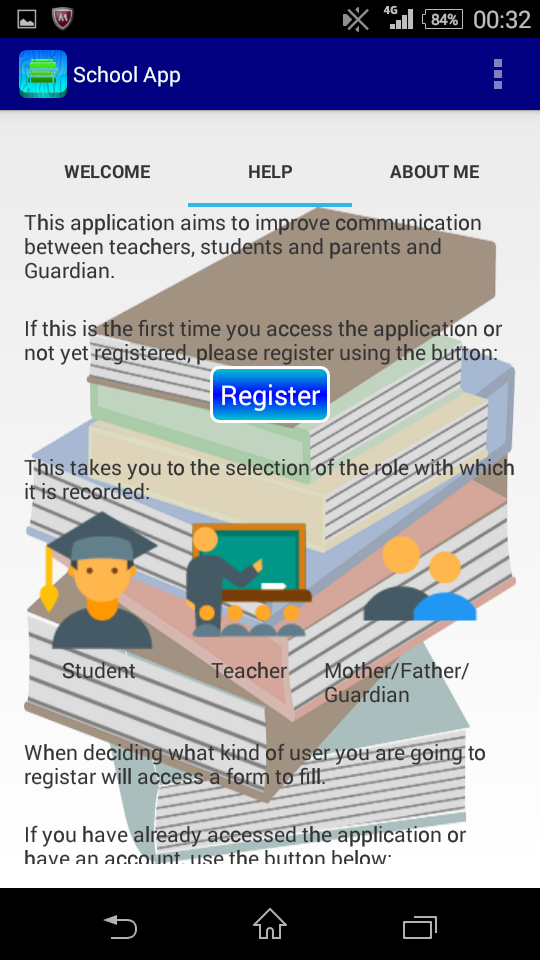
\includegraphics[scale=0.2]{Imagenes/App/help}
				\caption{Pantalla de ayuda de la Aplicación.}
				\label{fig:help}
			\end{figure}
		
		\subsection{Sobre mi (AboutMeFragment)}
			En la figura \ref{fig:aboutMe} se puede observar información referente al autor de la aplicación.
		
			\begin{figure}[h !]
				\centering
				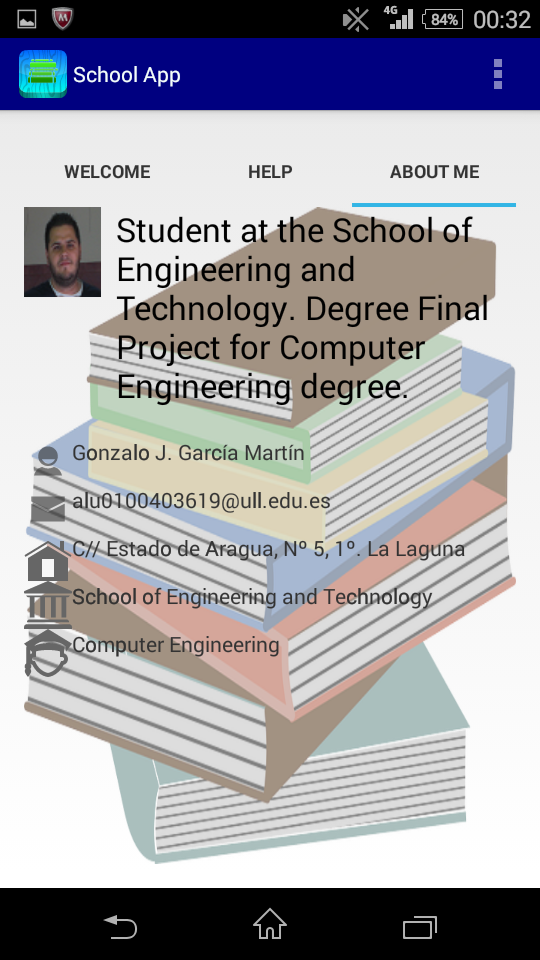
\includegraphics[scale=0.2]{Imagenes/App/aboutMe}
				\caption{Pantalla sobre el autor de la Aplicación.}
				\label{fig:aboutMe}
			\end{figure}
	
	\section{Cambio de idioma (ChangeLanguajeActivity)}
	
		En la figura \ref{fig:languaje} se puede observar los distintos idiomas disponibles de la aplicación. Al seleccionar uno de ellos y accionar el botón volver, quedará almacenado el idioma y las actividades lo cargarán al ser creadas.
	
		\begin{figure}[h !]
			\centering
			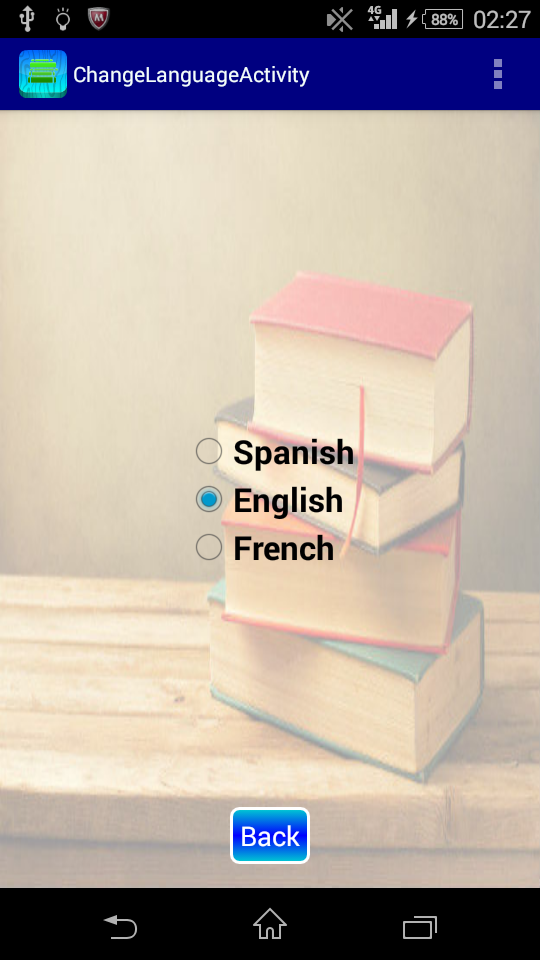
\includegraphics[scale=0.2]{Imagenes/App/ChangeLanguaje}
			\caption{Pantalla de cambio de idioma.}
			\label{fig:languaje}
		\end{figure}
			
	\section{Registro (RegisterActivity)} \label{sec:register}
		
		En la pantalla de registro (figura \ref{fig:register}) se pueden observar los perfiles con los que se puede registrar un usuario. Al seleccionar cualquiera de los tres botones, mostrará la pantalla de registro correspondiente.
		
		\begin{figure}[h !]
			\centering
			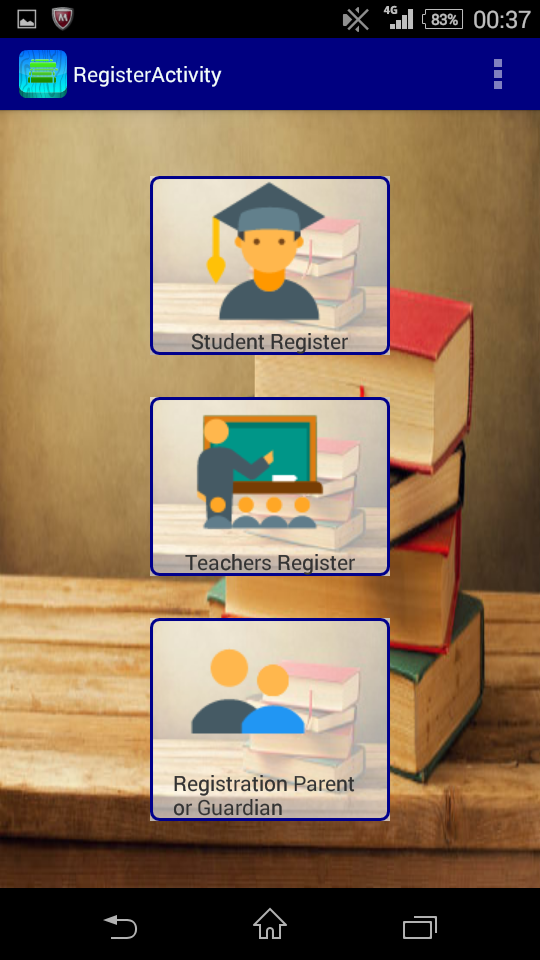
\includegraphics[scale=0.2]{Imagenes/App/registro}
			\caption{Pantalla de selección de perfil para el registro.}
			\label{fig:register}
		\end{figure}
		
		
		\subsection{Registro de alumnos (RegisterStudentActivity)} \label{sec:StudentRegister}
			
			La pantalla de registro de alumnos (figura \ref{fig:StudentRegister}) presenta un formulario que el usuario deberá rellenar. Presenta dos botones, uno que le devolverá a la pantalla de bienvenida (sección \ref{sec:welcome}) y otro que completará el registro. La aplicación solo permitirá el registro si se han rellenado todos los campos obligatorios. Una vez hecho, al accionar el botón, la aplicación llevará a cabo el registro del usuario en la base de datos de {\it Firebase}. También se accederá de forma automática a la aplicación.
			
			\begin{figure}[h !]
				\centering
				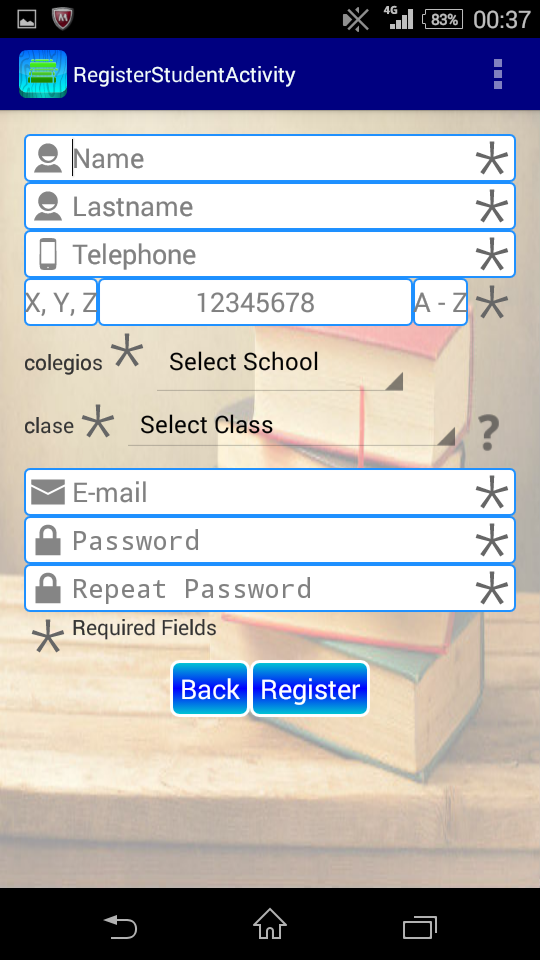
\includegraphics[scale=0.2]{Imagenes/App/registroAlumno}
				\caption{Registro de alumnos.}
				\label{fig:StudentRegister}
			\end{figure}
			
		\subsection{Registro de Profesores (RegisterTeacherActivity)}
		
			La pantalla de registro de profesor funciona exactamente igual que la pantalla de registro de alumno. Véase sección \ref{sec:StudentRegister}.
		
			\begin{figure}[h !]
				\centering
				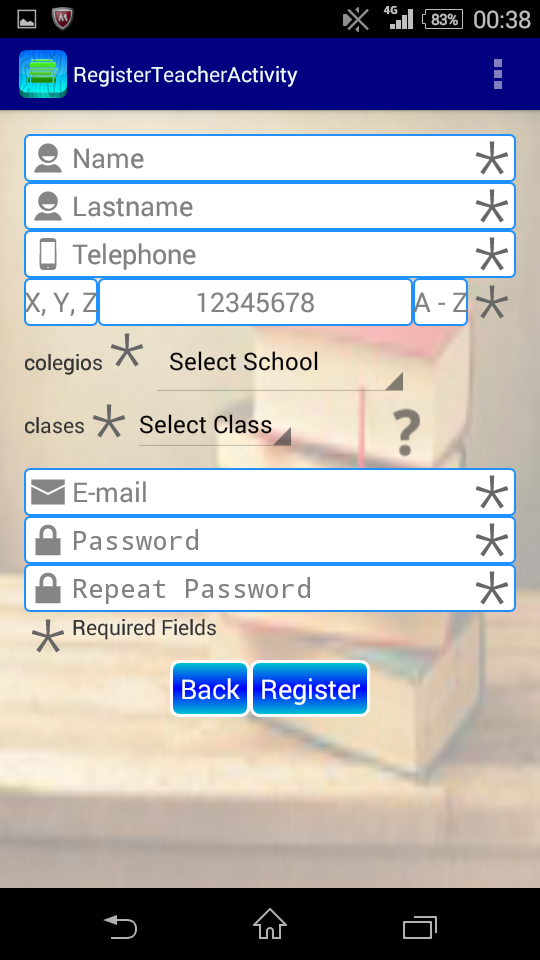
\includegraphics[scale=0.2]{Imagenes/App/registroProfe}
				\caption{Registro de profesores.}
				\label{fig:teacherRegister}
			\end{figure}
		
		\subsection{Registro de Padres (RegisterFatherActivity)} \label{sec:FatherRegister}
		
			La pantalla de registro de padre (figura \ref{fig:fatherRegister}) funciona exactamente igual que la de registro de alumnos, con la salvedad de que al usar el perfil de padre se debe al menos registrar un hijo para que el registro se lleve a cabo. Para llevar a cabo el registro de un hijo acciónese el botón con el símbolo de suma. Véase sección \ref{sec:addChild}.
			
			\begin{figure}[h !]
				\centering
				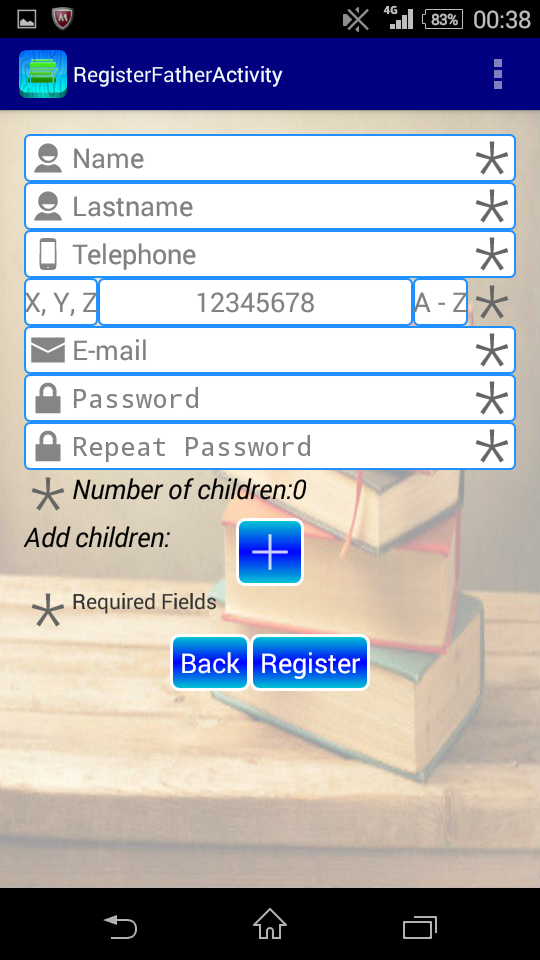
\includegraphics[scale=0.2]{Imagenes/App/registroPadre}
				\caption{Registro de padres.}
				\label{fig:fatherRegister}
			\end{figure}
			
		\subsection{Añadir hijo (AddChildActivity)} \label{sec:addChild}
			
			A esta pantalla (figura \ref{fig:addChildRegister}) se accede desde la pantalla de registro de padres (sección \ref{sec:FatherRegister}). Al introducir los datos del estudiante (sección \ref{sec:StudentRegister}), la aplicación consultará a la base de datos si existe el alumno. Si no existe se añadirá la información y se asociará con el padre, mientras que si existe solo se asociará. Tras el registro del alumno volverá a mostrar la pantalla de registro de padres (sección \ref{sec:FatherRegister}).
			
			\begin{figure}[h !]
				\centering
				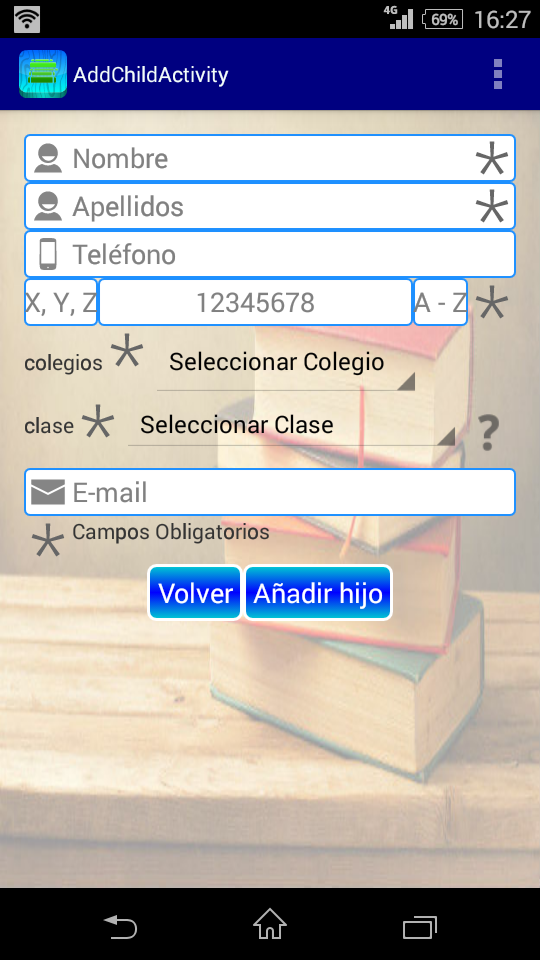
\includegraphics[scale=0.2]{Imagenes/App/addChild}
				\caption{Registro de hijos.}
				\label{fig:addChildRegister}
			\end{figure}
		
	\section{Acceso (LoginActivity)} \label{sec:login}
		
		En la pantalla de acceso (figura \ref{fig:login}) se puede observar que el usuario debe introducir su correo electrónico y contraseña para poder acceder a \CollegeApp con el botón de acceso. Si selecciona el de registro, se mostrará la pantalla de selección de perfil (Véase \ref{sec:register}). Para seleccionar {\it nueva contraseña} el usuario debe haber introducido previamente su correo electrónico. La aplicación se la solicitará al servidor de {\it Firebase} quien la mandará a la dirección con la que el usuario se ha registrado.  
		
		\begin{figure}[h !]
			\centering
			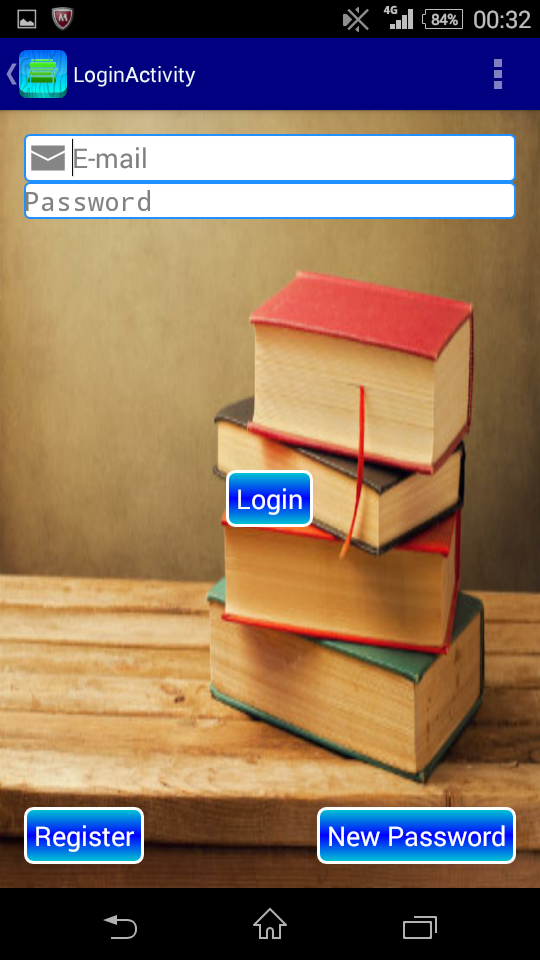
\includegraphics[scale=0.2]{Imagenes/App/login}
			\caption{Pantalla de acceso.}
			\label{fig:login}
		\end{figure}
		
		\bigskip
		En la figura \ref{fig:loginLand} se puede observar la pantalla de acceso con el dispositivo en horizontal.
		
		\begin{figure}[h !]
			\centering
			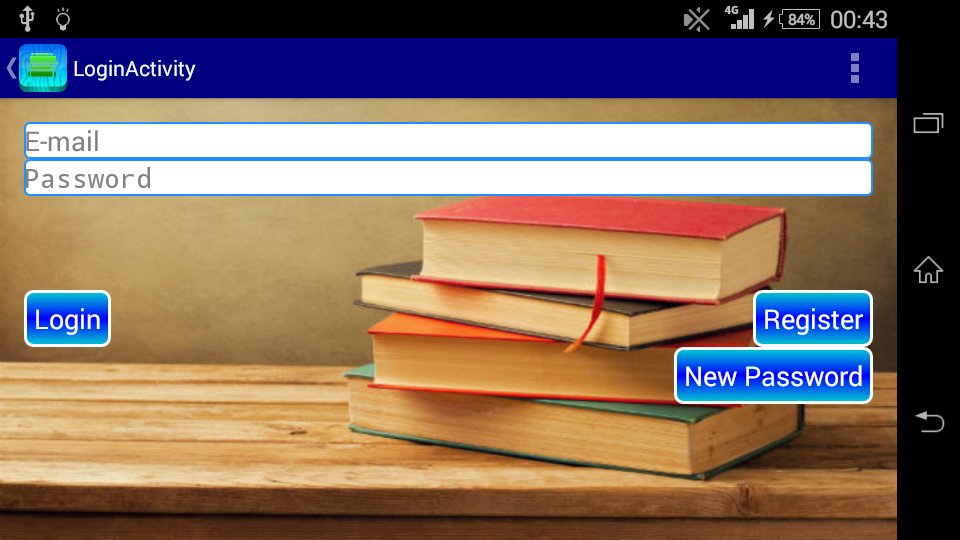
\includegraphics[scale=0.2]{Imagenes/App/loginLand}
			\caption{Pantalla de acceso con el dispositivo en horizontal.}
			\label{fig:loginLand}
		\end{figure}
		
	\section{Acceso como alumno (StudentTabActivity)}
		
		En esta pantalla se mostrarán en pestañas las listas de contactos de los usuarios con el perfil de alumno. También se mostrará una pestaña adicional para las notificaciones, es decir, mensajes que le lleguen al alumno (sección: \ref{sec:notifications}). En las opciones puede seleccionar cambiar sus datos (sección \ref{sec:myData}) y salir de la aplicación.
		Al seleccionar el botón citas (sección \ref{sec:dates}) se mostrará la pantalla encargada de añadir un evento al calendario del dispositivo. Esta funcionalidad viene implementada por el {\it sistema operativo}.
		
		\subsection{Lista de contactos: Alumnos (studentActivity)}
			
			En la figura \ref{fig:aluAlu} se puede observar los contactos que son compañeros de clase del alumno. Al seleccionar cualquiera de los contactos se podrá comunicar de forma directa con mensajes tipo chat (sección \ref{sec:chat}). Al hacer una selección larga podrá ver la información del contacto (sección \ref{sec:data}).
			
			\begin{figure}[h !]
				\centering
				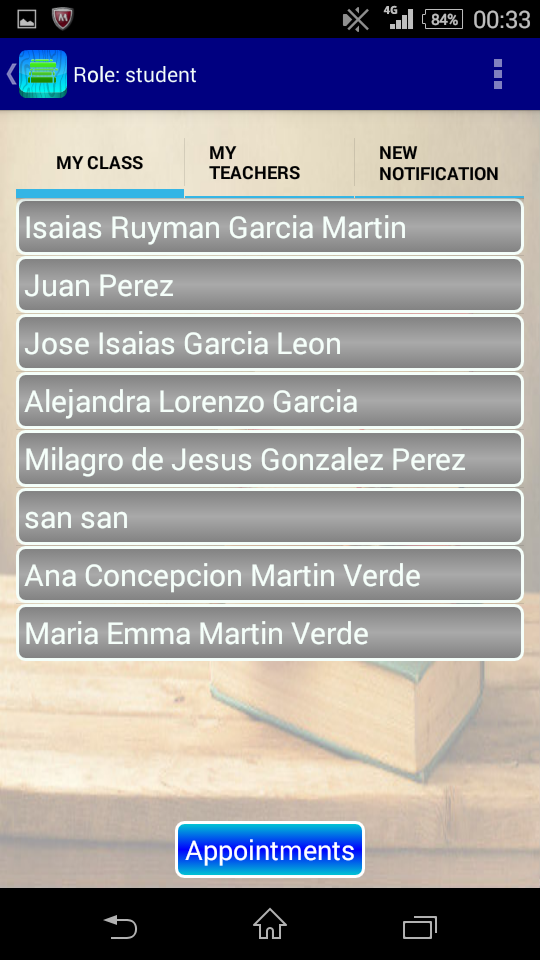
\includegraphics[scale=0.2]{Imagenes/App/aluAlu}
				\caption{Lista de contacto de alumnos para el perfil de alumno.}
				\label{fig:aluAlu}
			\end{figure}
			
		\subsection{Lista de contactos: Profesores (TeachersActivity)}
		
			En esta pantalla (figura \ref{fig:aluProfe}) se pueden ver los contactos que son profesores y le dan clase al usuario. Al seleccionar cualquiera de los contactos se podrá comunicar de forma directa con mensajes tipo chat (sección \ref{sec:chat}). Al hacer una selección larga podrá ver la información del contacto (sección \ref{sec:data}).
		
			\begin{figure}[h !]
				\centering
				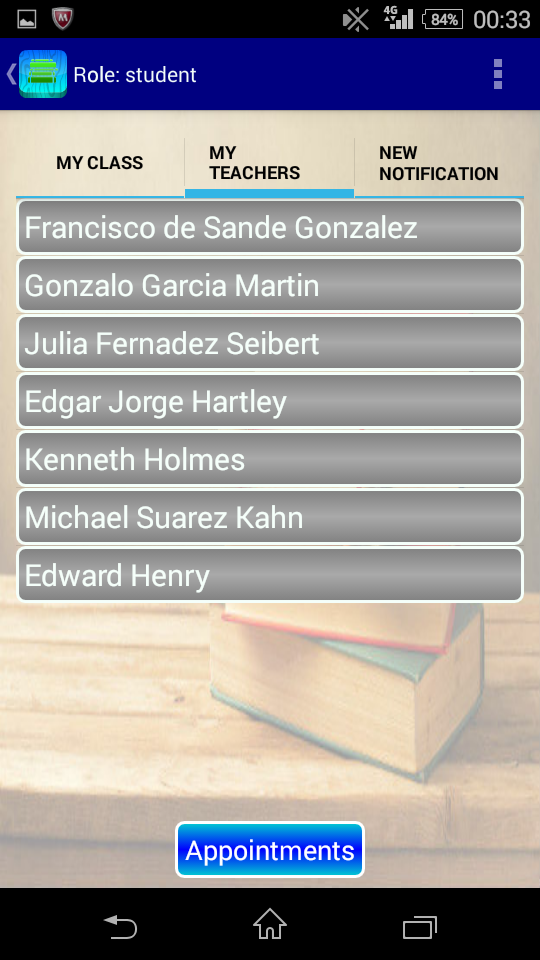
\includegraphics[scale=0.2]{Imagenes/App/aluProfe}
				\caption{Lista de contacto de profesores para el perfil de alumno.}
				\label{fig:aluProfe}
			\end{figure}
		
	\section{Acceso como padre (FatherTabActivity)}
	
		En esta pantalla se mostrarán en pestañas las listas de contactos de los usuarios con el perfil de padre. También se mostrará una pestaña adicional para las notificaciones, es decir, mensajes que le lleguen al padre (sección: \ref{sec:notifications}). En las opciones puede seleccionar cambiar sus datos (sección \ref{sec:myData}) y salir de la aplicación.
		Al seleccionar el botón citas (sección \ref{sec:dates}) se mostrará la pantalla encargada de añadir un evento al calendario del dispositivo. Esta funcionalidad viene implementada por el {\it sistema operativo}.
		
		\subsection{Lista de contactos: Padres (ExpandableFathersActivity)}
		
			En la figura \ref{fig:padrePadre} se puede observar la lista de contactos de padres para los usuarios con el mismo perfil. Estarán organizados según las clases en las que tengan algún hijo. Al seleccionar cualquier contacto se podrá comunicar de forma directa con mensajes tipo chat (sección \ref{sec:chat}). Al hacer una selección larga podrá ver la información del contacto (sección \ref{sec:data}).
			
			\begin{figure}[h !]
				\centering
				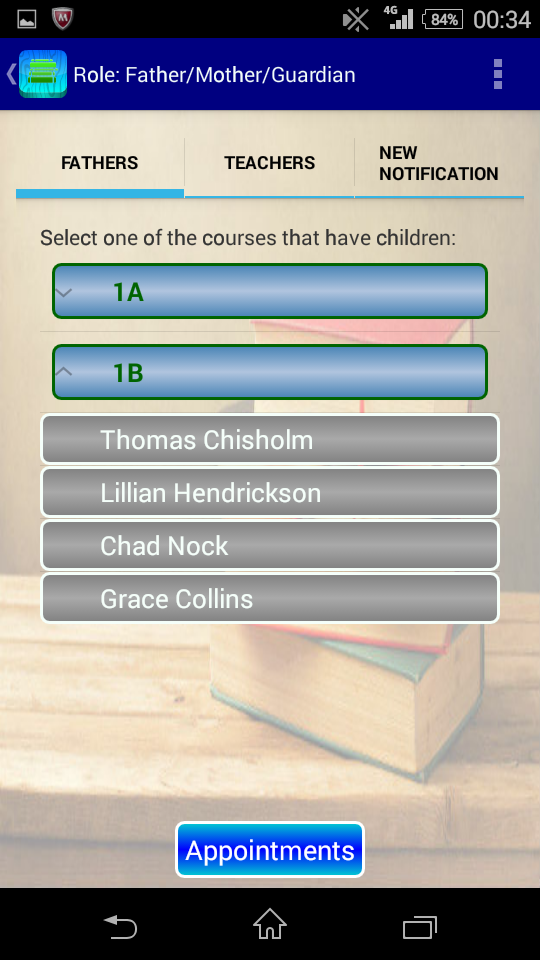
\includegraphics[scale=0.2]{Imagenes/App/padrePadre}
				\caption{Lista de contacto de padres para el perfil de padre.}
				\label{fig:padrePadre}
			\end{figure}
		
		\subsection{Lista de contactos: Profesores (ExpandableTeachersActivity)}
		
			En esta pantalla (figura \ref{fig:padreProfe}) se puede observar la lista de contactos de profesores para los usuarios con el perfil de padre. Estarán organizados según los profesores que den clases en las clases en las que tengan algún hijo. Al seleccionar cualquiera de los contactos se podrá comunicar de forma directa con mensajes tipo chat (sección \ref{sec:chat}). Al hacer una selección larga podrá ver la información del contacto (sección \ref{sec:data}).
		
			\begin{figure}[h !]
				\centering
				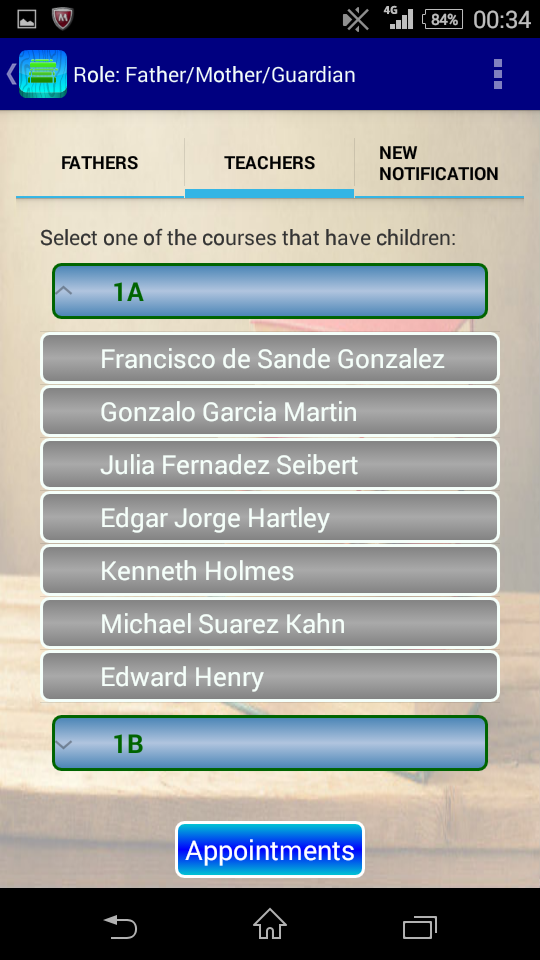
\includegraphics[scale=0.2]{Imagenes/App/padreProfe}
				\caption{Lista de contacto de profesores para el perfil de padre.}
				\label{fig:padreProfe}
			\end{figure}
		
	\section{Acceso como profesor (TeacherTabActivity)}
	
		En esta pantalla se mostrarán en pestañas las listas de contactos de los usuarios con el perfil de profesor. También se mostrará una pestaña adicional para las notificaciones, es decir, mensajes que le lleguen al padre (sección: \ref{sec:notifications}). En las opciones puede seleccionar cambiar sus datos (sección \ref{sec:myData}) y salir de la aplicación.
		Al seleccionar el botón citas (sección \ref{sec:dates}) se mostrará la pantalla encargada de añadir un evento al calendario del dispositivo. Esta funcionalidad viene implementada por el {\it sistema operativo}. Si se selecciona el botón de circulares, mostrará la pantalla para enviar el mismo mensaje a toda la clase (sección \ref{sec:circulares}).
		
		\subsection{Lista de contactos: Profesores (ExpandableTeachersActivity)}
		
			En esta pantalla (figura \ref{fig:profeProfe}) se mostrarán los compañeros de trabajo que enseñen a los alumnos a los que el da clase. Al seleccionar cualquiera de los contactos se podrá comunicar de forma directa con mensajes tipo chat (sección \ref{sec:chat}). Al hacer una selección larga podrá ver la información del contacto (sección \ref{sec:data}).
			
			\begin{figure}[h !]
				\centering
				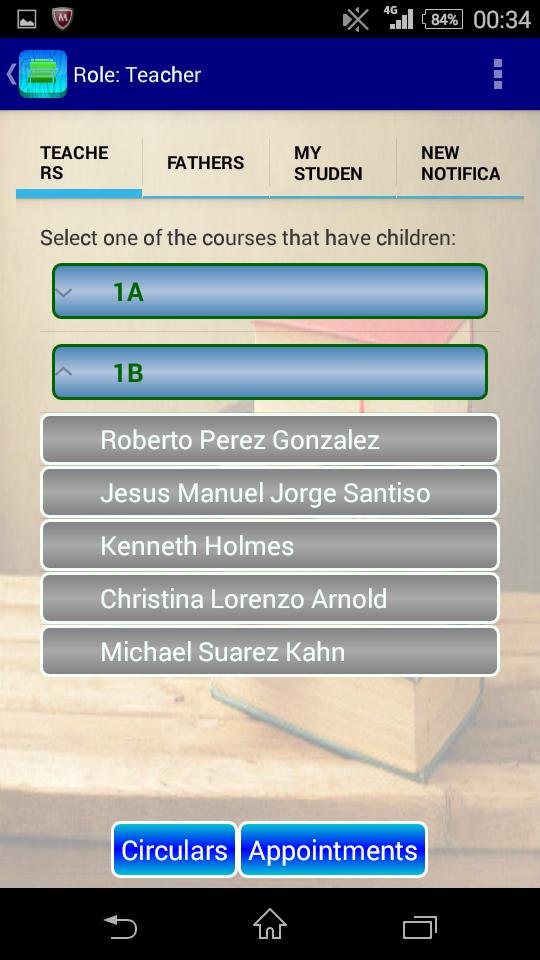
\includegraphics[scale=0.2]{Imagenes/App/profeProfe}
				\caption{Lista de contacto de profesores para el perfil de profesor.}
				\label{fig:profeProfe}
			\end{figure}
		
		\subsection{Lista de contactos: Padres (ExpandableFathersActivity)}
		
			En la figura \ref{fig:profePadre} se puede observar los contactos que son padres de alumnos a los que imparte clase. Al seleccionar cualquiera de los contactos se podrá comunicar de forma directa con mensajes tipo chat (sección \ref{sec:chat}). Al hacer una selección larga podrá ver la información del contacto (sección \ref{sec:data}).
			
			\begin{figure}[h !]
				\centering
				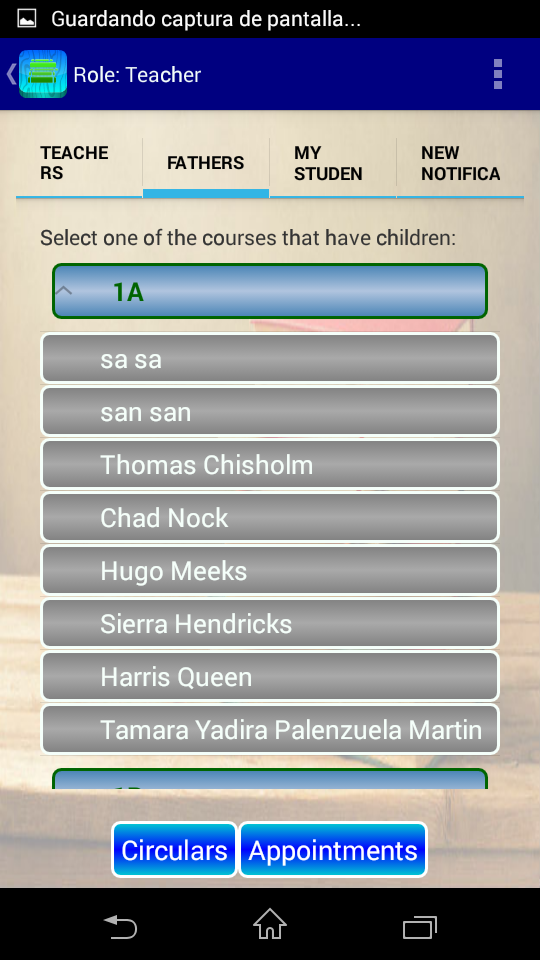
\includegraphics[scale=0.2]{Imagenes/App/profePadre}
				\caption{Lista de contacto de padres para el perfil de profesor.}
				\label{fig:profePadre}
			\end{figure}
		
		\subsection{Lista de contactos: Alumnos (ExpandableAlumnosActivity)}
		
			En esta pantalla (figura \ref{fig:profeAlu}) se mostrarán los alumnos a los que un profesor imparte clase. Al seleccionar cualquiera de los contactos se podrá comunicar de forma directa con mensajes tipo chat (sección \ref{sec:chat}). Al hacer una selección larga podrá ver la información del contacto (sección \ref{sec:data}).
		
			\begin{figure}[h !]
				\centering
				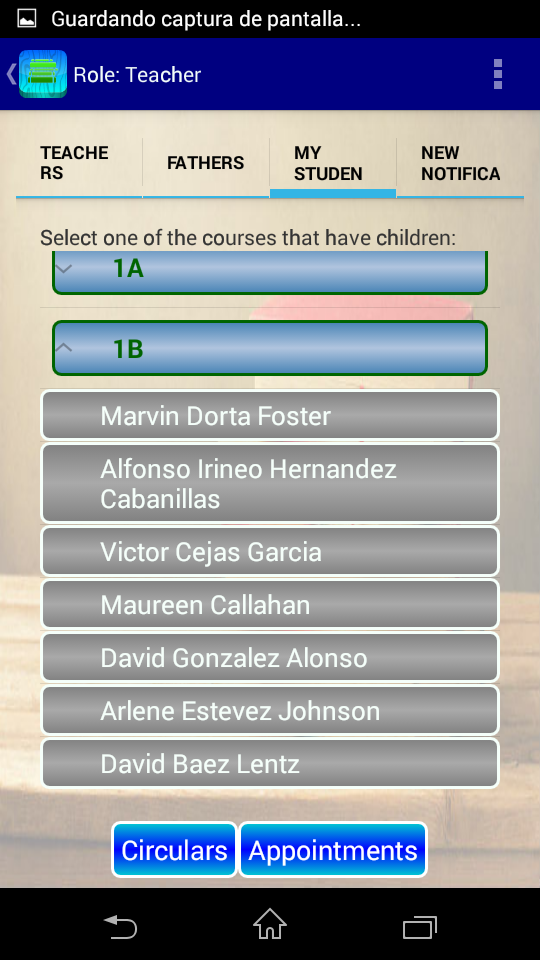
\includegraphics[scale=0.2]{Imagenes/App/profeAlu}
				\caption{Lista de contacto de alumnos para el perfil de padre.}
				\label{fig:profeAlu}
			\end{figure}
		
	\section{Notificaciones (notificationsActivity)} \label{sec:notifications}
	
		En la figura \ref{fig:notifications} se puede observar todas las notificaciones que reciben los usuarios. Estas son recuperadas y eliminadas de la base de datos en {\it Friebase}. La notificación muestra el nombre del remitente y el número de mensajes que ha enviado y que el usuario tiene sin leer. Se clasifican por colores según el perfil del usuario que las manda.
		Al seleccionar cualquiera se podrá comunicar de forma directa con mensajes tipo chat (sección \ref{sec:chat}) con el remitente.
	
		\begin{figure}[h !]
			\centering
			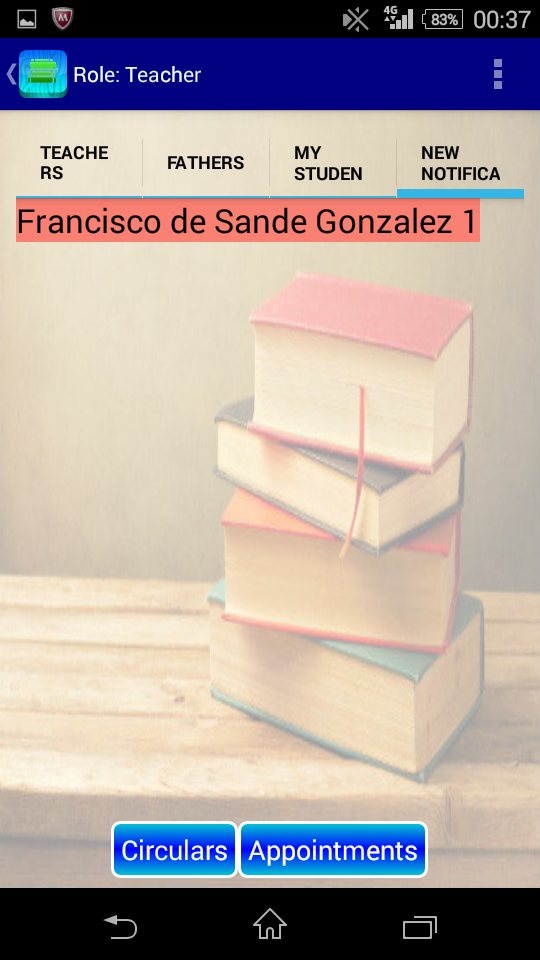
\includegraphics[scale=0.2]{Imagenes/App/Notifications}
			\caption{Notificaciones recibidas por los usuarios.}
			\label{fig:notifications}
		\end{figure}
	
	\section{Chat (ChatActivity)} \label{sec:chat}
	
		En esta pantalla (figura \ref{fig:chat}) obtenemos mensajería directa tipo chat con cualquiera de los contactos del usuario. Estos mensajes se guardan en la base de datos de {\it Firebase} de donde son recuperados y eliminados. También se guardan en una base de datos local, almacenada en el dispositivo. Si accedemos a las opciones podemos vaciar la conversación.
	
		\begin{figure}[h !]
			\centering
			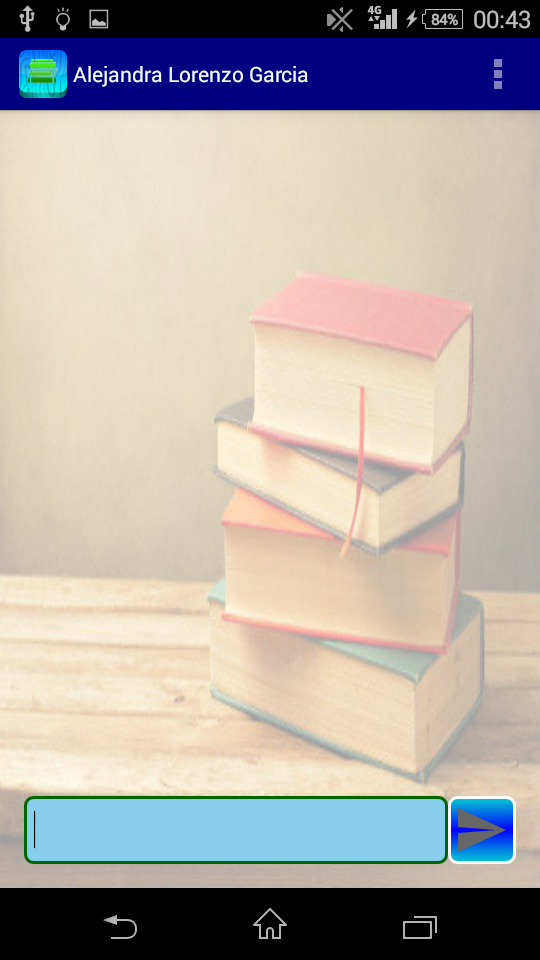
\includegraphics[scale=0.2]{Imagenes/App/chat}
			\caption{Mensajería tipo chat.}
			\label{fig:chat}
		\end{figure}
	
	\section{Mis Datos (MyDataActivity)} \label{sec:myData}
	
		En la figura \ref{fig:myData} se puede observar que el usuario puede ver los datos con los que se registró. Al seleccionar el botón modificar, podrá cambiar sus datos salvo el D.N.I y el correo electrónico. Si selecciona guardar se modificará la base de datos en el proveedor de servicios.
		Su selecciona dar de baja su cuenta, se borrará la información que hay en {\it Firebase}. También puede cambiar su contraseña con el botón destinado a ello (sección \ref{sec:changePassword}).
		
		\begin{figure}[h !]
			\centering
			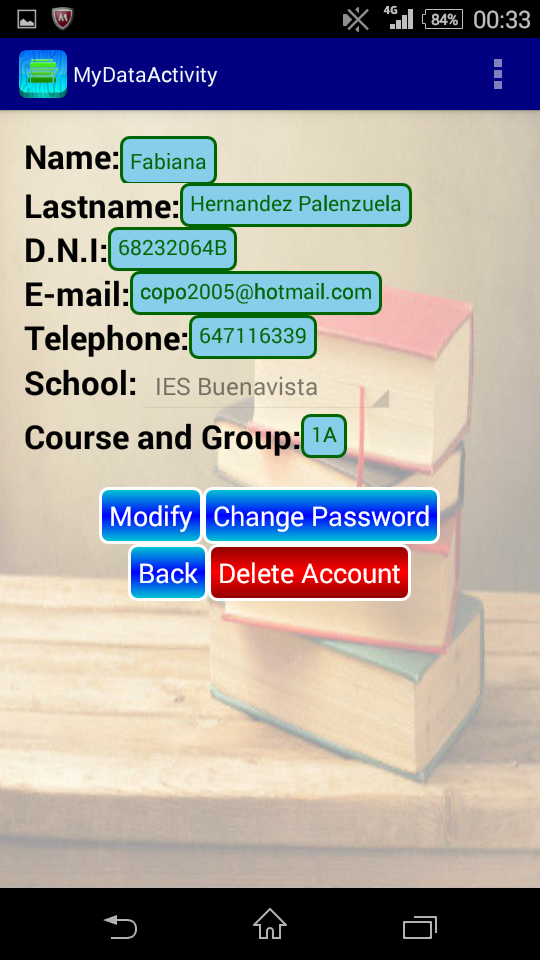
\includegraphics[scale=0.2]{Imagenes/App/myData}
			\caption{Datos del usuario.}
			\label{fig:myData}
		\end{figure}
	
	\section{Cambio de Contraseña (ChangePasswordactivity)} \label{sec:changePassword}
	
		En la pantalla de cambio de contraseña el usuario podrá cambiar su contraseña introduciendo su correo electrónico y contraseña antigua. También deberá seleccionar una nueva contraseña y repetirla. Si desea hacer el cambio permanente solo deberá accionar el botón guardar.
	
		\begin{figure}[h !]
			\centering
			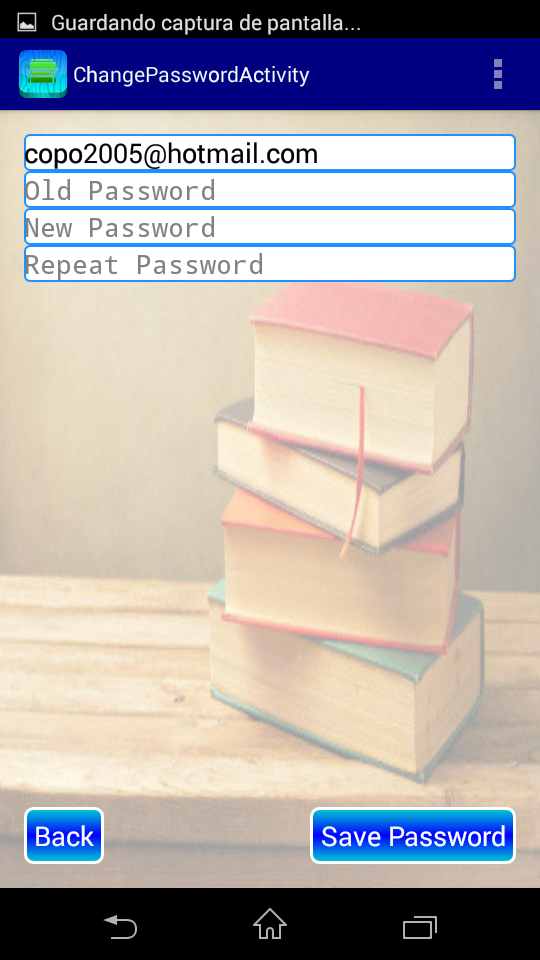
\includegraphics[scale=0.2]{Imagenes/App/changePassword}
			\caption{Cambio de contraseña.}
			\label{fig:changePassword}
		\end{figure}
	
	\section{Circulares (CircularesActivity)} \label{sec:circulares}
	
		En esta pantalla (figura \ref{fig:circulares}) se podrá mandar un mismo mensaje a una o varias clases, ya sean alumnos o padres. Al seleccionar el botón enviar, se mandará el mismo mensaje a cada uno de los alumnos que pertenezca a la clase seleccionada.
	
		\begin{figure}[h !]
			\centering
			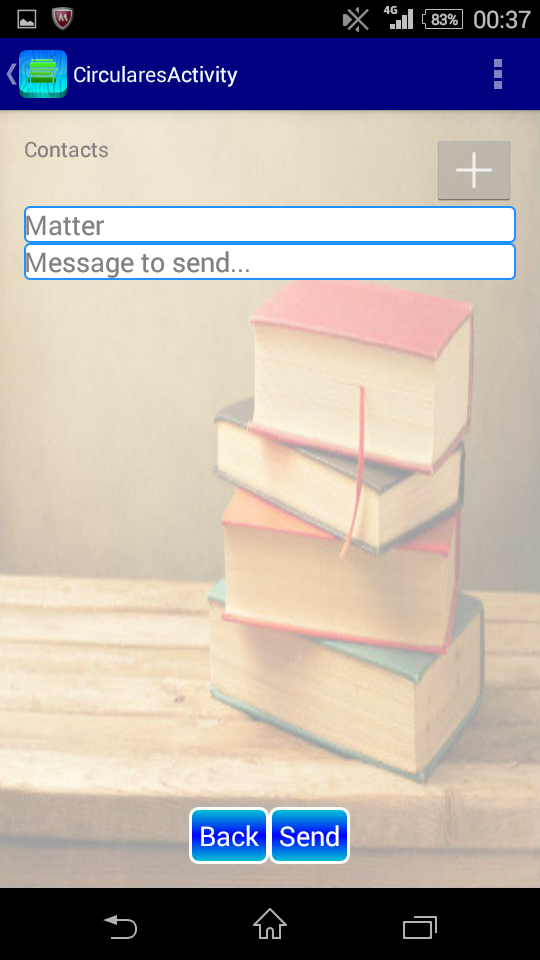
\includegraphics[scale=0.2]{Imagenes/App/Circulares}
			\caption{Pantalla de circulares.}
			\label{fig:circulares}
		\end{figure}
		
		En la figura \ref{fig:selectClass} se puede observar cómo se seleccionan las clases.
		
		\begin{figure}[h !]
			\centering
			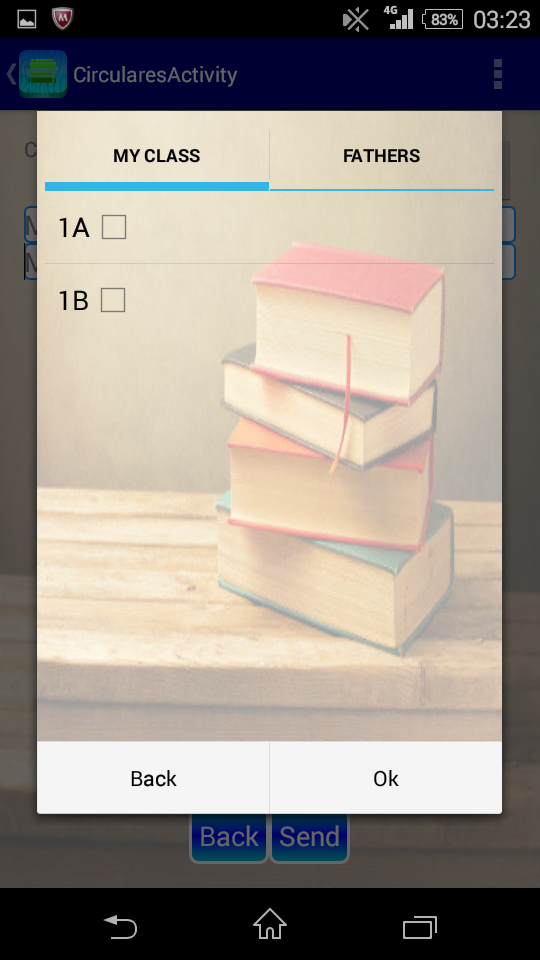
\includegraphics[scale=0.2]{Imagenes/App/selectClass}
			\caption{Pantalla de circulares, seleccionar clase.}
			\label{fig:selectClass}
		\end{figure}
	
	\section{Citas} \label{sec:dates}
		Esta funcionalidad (figura \ref{fig:addEvent}) usa el calendario del dispositivo. Lanza la actividad que permite añadir eventos. Viene implementado en el {\it sistema operativo}.
		Se introducen los datos en los campos correspondientes y luego se selecciona guardar. Se puede elegir el calendario en el que guardar el evento, en el dispositivo o en el de {\it Google}.
		
			\begin{figure}[h !]
				\centering
				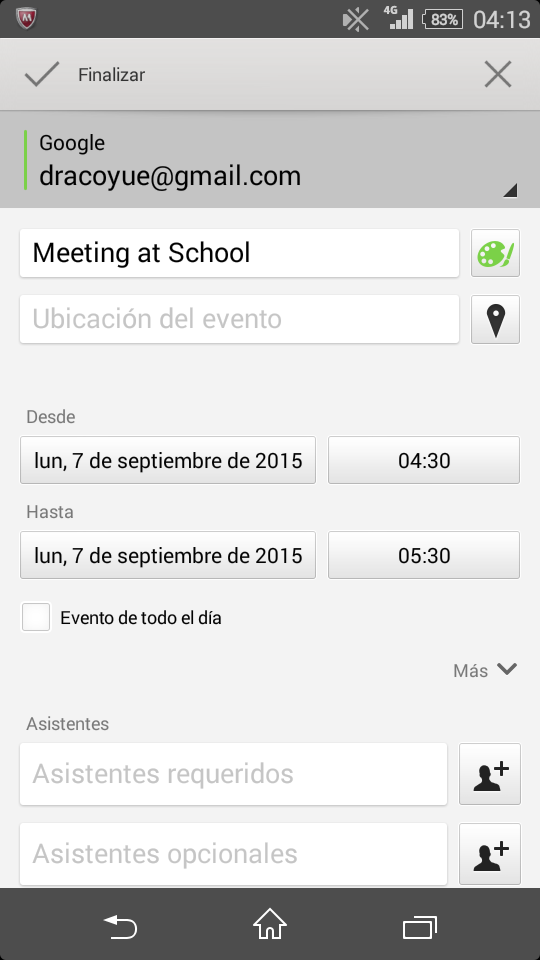
\includegraphics[scale=0.2]{Imagenes/App/addEvent}
				\caption{añadir evento al calendario.}
				\label{fig:addEvent}
			\end{figure}
	
	\section{Datos del contacto (DataActivity)} \label{sec:data}
	
		En esta pantalla (figura \ref{fig:data}) se muestran los datos de cualquier contacto del usuario.
		
		\begin{figure}[h !]
			\centering
			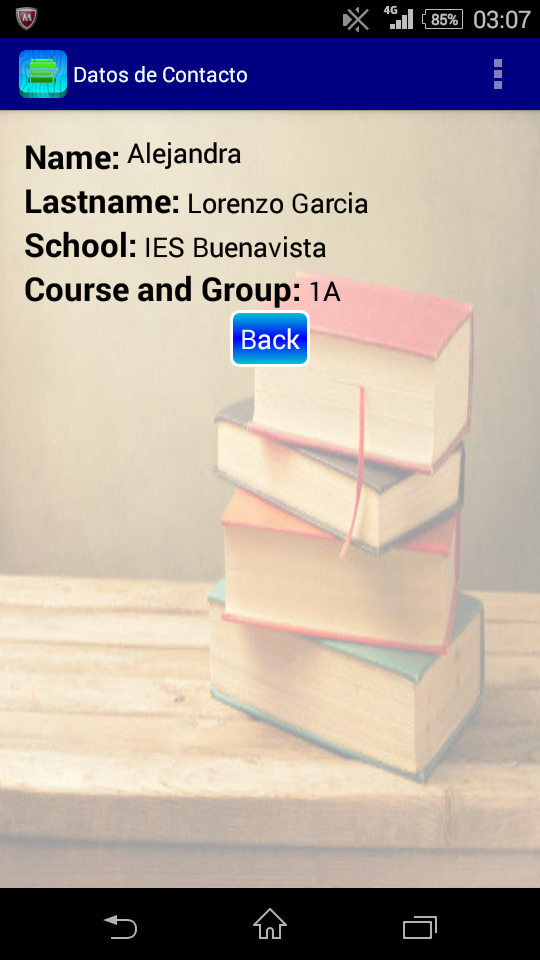
\includegraphics[scale=0.2]{Imagenes/App/dataContact}
			\caption{Pantalla de datos de un contacto.}
			\label{fig:data}
		\end{figure}